%
% Licensed to the OpenAirInterface (OAI) Software Alliance under one or more
% contributor license agreements.  See the NOTICE file distributed with
% this work for additional information regarding copyright ownership.
% The OpenAirInterface Software Alliance licenses this file to You under
% the OAI Public License, Version 1.1  (the "License"); you may not use this file
% except in compliance with the License.
% You may obtain a copy of the License at
%
%      http://www.openairinterface.org/?page_id=698
%
% Unless required by applicable law or agreed to in writing, software
% distributed under the License is distributed on an "AS IS" BASIS,
% WITHOUT WARRANTIES OR CONDITIONS OF ANY KIND, either express or implied.
% See the License for the specific language governing permissions and
% limitations under the License.
%-------------------------------------------------------------------------------
% For more information about the OpenAirInterface (OAI) Software Alliance:
%      contact@openairinterface.org
%

\documentclass{article}

\usepackage[a4paper, total={6in, 8in}]{geometry}

\usepackage{amsmath}
\usepackage{amsfonts}
\usepackage{amssymb}
\usepackage{booktabs}
\usepackage{url}
\usepackage{tcolorbox}

\usepackage{tikz}
\usetikzlibrary{arrows,decorations,shapes,backgrounds,patterns}
\usepackage{pgfplots}
\pgfplotsset{compat=newest}
\definecolor{green}{RGB}{32,127,43}
\usetikzlibrary{calc}

\usepackage{listings}
\lstdefinestyle{customc}{
  belowcaptionskip=1\baselineskip,
  breaklines=true,
  frame=L,
  xleftmargin=\parindent,
  language=C,
  showstringspaces=false,
  basicstyle=\footnotesize\ttfamily,
  keywordstyle=\bfseries\color{green!40!black},
  commentstyle=\itshape\color{purple!40!black},
  identifierstyle=\color{blue},
  stringstyle=\color{orange},
}
\lstset{escapechar=@,style=customc}

\title{NR LDPC Decoder}
\author{Sebastian Wagner (TCL)}
\date{\today}

\def\0{\mathbf{0}}
\def\b{\mathbf{b}}
\def\Bbb{\mathbb{B}}
\def\Bcal{\mathcal{B}}
\def\c{\mathbf{c}}
\def\C{\mathbf{C}}
\def\Cbb{\mathbb{C}}
\def\Ccal{\mathcal{C}}
\def\eqdef{\triangleq}
\def\g{\mathbf{g}}
\def\G{\mathbf{G}}
\def\Gcal{\mathcal{G}}
\def\h{\mathbf{h}}
\def\H{\mathbf{H}}
\def\Hbg{\mathbf{H}_\mathrm{BG}}
\def\Hbgo{\mathbf{H}_\mathrm{BG1}}
\def\Hbgt{\mathbf{H}_\mathrm{BG2}}
\def\I{\mathbf{I}}
\def\Kb{{K_b}}
\def\m{\mathbf{m}}
\def\Mb{{M_b}}
\def\Nb{{N_b}}
\def\Nbb{\mathbb{N}}
\def\n{\mathbf{n}}
\def\nr{{n_{\rm r}}}
\def\nt{{n_{\rm t}}}
\def\s{\mathbf{s}}
\def\SNR{\mathsf{SNR}}
\def\y{\mathbf{y}}
\def\z{\mathbf{z}}
\def\Z{\mathbf{Z}}
\def\Zc{{Z_c}}


\def\herm{\mathsf{H}}
\def\trans{\mathsf{T}}
\def\EE{\mathsf{E}}
\newcommand{\sgn}{\operatorname{sgn}}

\begin{document}

\maketitle

\begin{tikzpicture}[remember picture,overlay]
   \node[anchor=north west,inner sep=0pt] at (current page.north west)
              {
\includegraphics[scale=0.5]{logo.png}};
\end{tikzpicture}


\begin{center}Currently Supported:\end{center}
\tcbox[center]{
    \begin{tabular}{lll}
      \toprule
      \textbf{BG} & \textbf{Lifting Size Z} & \textbf{Code Rate R} \\
      \midrule
        1 & all & 1/3, 2/3, 8/9 \\
        2 & all & 1/5, 1/3, 2/3 \\
      \bottomrule
    \end{tabular}
}

\tableofcontents

\newpage
\section{Introduction}
\label{sec:introduction}

Low Density Parity Check (LDPC) codes have been developed by Gallager in 1963 \cite{gallager1962low}. They are linear error correcting codes that are capacity-achieving for large block length and are completely described by their Parity Check Matrix (PCM) $\H^{M\times N}$. The PCM $\H$ defines $M$ constraints on the codeword $\c$ of length $N$ such that
\begin{equation}
  \label{eq:29}
  \H\c = \0.
\end{equation}
The number of information bits $B$ that can be encoded with $\H$ is given by $B=N-M$. Hence the code rate $R$ of $\H$ reads
\begin{equation}
  \label{eq:37}
  R = \frac{B}{N} = 1-\frac{M}{N}.
\end{equation}


\subsection{LDPC in NR}
\label{sec:ldpc-nr}

NR uses quasi-cyclic (QC) Protograph LDPC codes, i.e. a smaller graph, called Base Graph (BG), is defined and utilized to construct the larger PCM. This has the advantage that the large PCM does not have to be stored in memory and allows for a more efficient implementation while maintaining good decoding properties.
Two BGs $\Hbg\in\Nbb^{\Mb\times \Nb}$ are defined in NR:
\begin{enumerate}
\item $\Hbgo\in\Nbb^{46\times 68}$
\item $\Hbgt\in\Nbb^{42\times 52}$
\end{enumerate}
where $\Nbb$ is the set of integers. For instance the first 3 rows and 13 columns of BG2 are given by

\setcounter{MaxMatrixCols}{30}
\begin{equation*}
  \label{eq:33}
  \Hbgt =
  \begin{bmatrix}
    9   & 117       & 204       & 26  & \emptyset & \emptyset & 189       & \emptyset & \emptyset & 205       & 0         & 0         & \emptyset & \emptyset \\
    127 & \emptyset & \emptyset & 166 & 253       & 125       & 226       & 156       & 224       & 252       & \emptyset & 0         & 0         & \emptyset \\
    81  & 114       & \emptyset & 44  & 52        & \emptyset & \emptyset & \emptyset & 240       & \emptyset & 1         & \emptyset & 0         & 0
  \end{bmatrix}.
\end{equation*}

To obtain the PCM $\H$ from the BG $\Hbg$, each element $\Hbg(i,j)$ in the BG is replaced by a lifting matrix of size $\Zc\times \Zc$ according to
\begin{equation}
  \label{eq:35}
  \Hbg(i,j) =
  \begin{cases}
    \0 & \textrm{if}~ \Hbg(i,j)=\emptyset \\
    \I_{P_{ij}} & \textrm{otherwise}
  \end{cases}
\end{equation}
where $\I_{P_{ij}}$ is the identity matrix circularly shifted to the right by $P_{ij} = \Hbg(i,j)\mod \Zc$. Hence, the resulting PCM $\H$ will be of size $\Mb\Zc\times\Nb\Zc$.

The lifting size $\Zc$ depends on the number of bits to encode. To limit the complexity, a discrete set $\mathcal{Z}$ of possible values of $\Zc$ has been defined in \cite{3gpp2017_38212} and the optimal value $\Zc$ is calculated according to
\begin{equation}
  \label{eq:36}
  \Zc = \min_{\Z\in\mathcal{Z}}\left[Z\geq\frac{B}{\Nb}\right].
\end{equation}

The base rate of the two BGs is $1/3$ and $1/5$ for BG1 and BG2, respectively. That is, BG1 encodes $K=22\Zc$ bits and BG2 encodes $K=10\Zc$ bits. Note that the first 2 columns of BG 1 and 2 are always punctured, that is after encoding, the first $2\Zc$ bits are discarded and not transmitted.
For instance, consider $B=500$ information bits to encode using BG2, \eqref{eq:36} yields $\Zc=64$ hence $K=640$. Since $K>B$, $K-B=140$ filler bits are appended to the information bits. The PCM $\Hbgt$ is of size $2688\times 3328$ and the $640$ bits $\b$ are encoded according to \eqref{eq:29} at a rate $R \approx 0.192$. To achieve the higher base rate of $0.2$, the first $128$ are punctured, i.e. instead of transmitting all $3328$ bits, only $3200$ are transmitted resulting in the desired rate $R=640/3200=0.2$.

\subsection{LDPC Decoding}
\label{sec:ldpc-decoding}

The decoding of codeword $\c$ can be achieved via the classical message passing algorithm. This algorithm can be illustrated best using the Tanner graph of the PCM. The rows of the PCM are called check nodes (CN) since they represent the parity check equations. The parity check equation of each of these check nodes involves various bits in the codeword. Similarly, every column of the PCM corresponds to a bit and each bit is involved in several parity check equations. In the Tanner graph representation, the bits are called bit nodes (BN). Let's go back to the previous example of BG2 and assume $\Zc=2$, hence the first 3 rows and 13 columns of BG2 $\Hbgt$ read
\begin{equation*}
  \label{eq:36}
  \Hbgt =
  \begin{bmatrix}
    1 & 1         & 0         & 0 & \emptyset & \emptyset & 1         & \emptyset & \emptyset & 1         & 0         & 0         & \emptyset & \emptyset \\
    1 & \emptyset & \emptyset & 0 & 1         & 1         & 0         & 0         & 0         & 0         & \emptyset & 0         & 0         & \emptyset \\
    1 & 0         & \emptyset & 0 & 0         & \emptyset & \emptyset & \emptyset & 0         & \emptyset & 1         & \emptyset & 0         & 0
  \end{bmatrix}.
\end{equation*}
Replacing the elements according to \eqref{eq:35}, we obtain the first 6 rows and 26 columns of the PCM as
\begin{equation*}
  \label{eq:39}
  \H =
  \begin{bmatrix}
    0 & 1 & 0 & 1 & 1 & 0 & 1 & 0 & 0 & 0 & 0 & 0 & 0 & 1 & 0 & 0 & 0 & 0 & 0 & 1 & 1 & 0 & 1 & 0 & 0 & 0 & 0 & 0\\
    1 & 0 & 1 & 0 & 0 & 1 & 0 & 1 & 0 & 0 & 0 & 0 & 1 & 0 & 0 & 0 & 0 & 0 & 1 & 0 & 0 & 1 & 0 & 1 & 0 & 0 & 0 & 0\\
    0 & 1 & 0 & 0 & 0 & 0 & 1 & 0 & 0 & 1 & 0 & 1 & 1 & 0 & 1 & 0 & 1 & 0 & 1 & 0 & 0 & 0 & 1 & 0 & 1 & 0 & 0 & 0\\
    1 & 0 & 0 & 0 & 0 & 0 & 0 & 1 & 1 & 0 & 1 & 0 & 0 & 1 & 0 & 1 & 0 & 1 & 0 & 1 & 0 & 0 & 0 & 1 & 0 & 1 & 0 & 0\\
    0 & 1 & 1 & 0 & 0 & 0 & 1 & 0 & 1 & 0 & 0 & 0 & 0 & 0 & 0 & 0 & 1 & 0 & 0 & 0 & 0 & 1 & 0 & 0 & 1 & 0 & 1 & 0\\
    1 & 0 & 0 & 1 & 0 & 0 & 0 & 1 & 0 & 1 & 0 & 0 & 0 & 0 & 0 & 0 & 0 & 1 & 0 & 0 & 1 & 0 & 0 & 0 & 0 & 1 & 0 & 1
  \end{bmatrix}.
\end{equation*}

The Tanner graph of the first 8 BNs is shown in Figure \ref{fig:tannergraph}.

\begin{figure}[ht]
  \label{fig:tannergraph}
  \centering
  \def\ww{0.3cm}
  \def\hh{0.3cm}
  \tikzstyle{cnode}=[fill=white,rectangle,draw=black,thick,inner sep=2pt, minimum height=\hh,minimum width=\ww, rounded corners=1pt,text width=\ww]
  \tikzstyle{vnode}=[fill=white,circle,draw=black,thick,inner sep=2pt, minimum height=\hh,minimum width=\ww, rounded corners=1pt,text width=\ww]
  \tikzstyle{connector}=[<->,>=latex',semithick]

  \begin{tikzpicture}
    \tikzstyle{every node}=[node distance=1.5cm,text centered]
    % Check nodes
    \node[cnode, label=above:$v_0$] (v0) {};
    \node[cnode, label=above:$v_1$, right of=v0] (v1) {};
    \node[cnode, label=above:$v_2$, right of=v1] (v2) {};
    % Variable nodes
    \node[vnode, label=below:$c_3$, below of=v1, node distance=1.5cm] (c3) {};
    \node[vnode, label=below:$c_2$, left of=c3, node distance=1.5cm] (c2) {};
    \node[vnode, label=below:$c_1$, left of=c2, node distance=1.5cm] (c1) {};
    \node[vnode, label=below:$c_0$, left of=c1, node distance=1.5cm] (c0) {};
    \node[vnode, label=below:$c_4$, right of=c3, node distance=1.5cm] (c4) {};
    \node[vnode, label=below:$c_5$, right of=c4, node distance=1.5cm] (c5) {};
    \node[vnode, label=below:$c_6$, right of=c5, node distance=1.5cm] (c6) {};

    % Draw edges
    \draw (c0) edge[connector] (v1);
    \draw (c1) edge[connector] (v0);
    \draw (c1) edge[connector] (v2);
    \draw (c2) edge[connector] (v1);
    \draw (c3) edge[connector] (v0);
    \draw (c4) edge[connector] (v0);
    \draw (c4) edge[connector] (v2);
    \draw (c5) edge[connector] (v1);
    \draw (c6) edge[connector] (v0);
    \draw (c6) edge[connector] (v2);

  \end{tikzpicture}

  \caption{Tanner graph for first 7 bits nodes and 3 check nodes from \eqref{eq:39}.}
\end{figure}

The message passing algorithm is an iterative algorithm where probabilities of the bits (being either 0 or 1) are exchanged between the BNs and CNs. After sufficient iterations, the probabilities will have either converged to either 0 or 1 and the parity check equations will be satisfied, at this point, the codeword has been decoded correctly.

\newpage
\section{LDPC Decoder Implementation}
\label{sec:ldpc-implementation}

The implementation on a general purpose processor (GPP) has to take advantage of potential instruction extension of the processor architecture. We focus on the Intel x86 instruction set architecture (ISA) and its advanced vector extension (AVX). In particular, we utilize AVX2 with its 256-bit single instruction multiple data (SIMD) format. In order to utilize AVX2 to speed up the processing at the CNs and BNs, the corresponding data has to be ordered/aligned in a specific way. The processing flow of the LDPC decoder is depicted in \ref{fig:ldpc_decoder_flow}.

\begin{figure}[ht]
  \label{fig:ldpc_decoder_flow}
  \centering
  \def\ww{0.3cm}
  \def\hh{0.3cm}
  \tikzstyle{func}=[,draw=none]
  \tikzstyle{connector}=[->,>=latex',semithick]

  \begin{tikzpicture}
    \tikzstyle{every node}=[node distance=2.5cm,text centered]
    % Check nodes
    % First iteration
    \node[func]                               (llr2llrProcBuf) {\texttt{llr2llrProcBuf}};
    \node[func, above of=llr2llrProcBuf]      (llr2CnProcBuf)  {\texttt{llr2CnProcBuf}};
    \node[func, above right of=llr2CnProcBuf] (cnProc1)        {\texttt{cnProc}};
    \node[func, below right of=cnProc1]       (cn2bnProcBuf1)  {\texttt{cn2bnProcBuf}};
    \node[func, below  of=cn2bnProcBuf1]      (bnProcPc1)      {\texttt{bnProcPc}};

    % Iterations
    \node[func, right of=cnProc1, node distance=7cm] (cnProc)       {\texttt{cnProc}};
    \node[func, below right of=cnProc]               (cn2bnProcBuf) {\texttt{cn2bnProcBuf}};
    \node[func, below of=cn2bnProcBuf]               (bnProcPc)     {\texttt{bnProcPc}};
    \node[func, below left of=cnProc]                (bn2cnProcBuf) {\texttt{bn2cnProcBuf}};
    \node[func, below  of=bn2cnProcBuf]              (bnProc)       {\texttt{bnProc}};

    % Post processing
    \node[func, below of=bnProcPc]      (llrRes2llrOut) {\texttt{llrRes2llrOut}};
    \node[func, below of=llrRes2llrOut, node distance=1cm] (llr2bit) {\texttt{llr2bit}};

    % Draw edges
    \draw (llr2llrProcBuf)  edge[connector] (llr2CnProcBuf);
    \draw (llr2CnProcBuf)   edge[connector] (cnProc1);
    \draw (cnProc1)         edge[connector] (cn2bnProcBuf1);
    \draw (cn2bnProcBuf1)   edge[connector] (bnProcPc1);

    \draw (bnProcPc)       edge[connector] (bnProc);
    \draw (bnProc)         edge[connector] (bn2cnProcBuf);
    \draw (bn2cnProcBuf)   edge[connector] (cnProc);
    \draw (cnProc)         edge[connector] (cn2bnProcBuf);
    \draw (cn2bnProcBuf)   edge[connector] (bnProcPc);

    \draw (bnProcPc1)      edge[connector] (bnProc);

    \draw (bnProcPc) edge[connector] node[left] {iterations done} (llrRes2llrOut);
    \draw (llrRes2llrOut) edge[connector] (llr2bit);

    % Boxes
    \node[inner sep=0pt,above right of=cn2bnProcBuf1, node distance = 2.5cm] (ref) {};

    \draw[fill=black,opacity=.2, rounded corners] (llr2llrProcBuf.south west) rectangle ($(ref) + (-.5cm,.5cm)$);
    \draw[fill=black,opacity=.2, rounded corners] ($(ref) + (.5cm,.5cm)$) rectangle ($(bnProcPc.south east) + (.4cm,0)$);

    \node[func, above of=cnProc1, node distance=.8cm] (iter1) {\textbf{First Iteration}};
    \node[func, above of=cnProc , node distance=.8cm] (iterX) {\textbf{Subsequent Iterations}};

  \end{tikzpicture}

  \caption{LDPC Decoder processing flow.}
\end{figure}

The functions involved are described in more detail in table \ref{tab:sum_func}.

\begin{table}[ht]
  \centering
  \begin{tabular}{ll}
    \toprule
    \textbf{Function} & \textbf{Description} \\
    \midrule
    \texttt{llr2llrProcBuf} & Copies input LLRs to LLR processing buffer \\
    \texttt{llr2CnProcBuf}  & Copies input LLRs to CN  processing buffer \\
    \texttt{cnProc}         & Performs CN signal processing \\
    \texttt{cn2bnProcBuf}   & Copies the CN results to the BN processing buffer \\
    \texttt{bnProcPc}       & Performs BN processing for parity check and/or hard-decision \\
    \texttt{bnProc}         & Utilizes the results of \texttt{bnProcPc} to compute LLRs for CN processing \\
    \texttt{bn2cnProcBuf}   & Copies the BN results to the CN processing buffer \\
    \texttt{llrRes2llrOut}  & Copies the results of \texttt{bnProcPc} to output LLRs \\
    \texttt{llr2bit}        & Performs hard-decision on the output LLRs \\
    \bottomrule
  \end{tabular}
  \caption{Summary of the LDPC decoder functions.}
  \label{tab:sum_func}
\end{table}

The input LLRs are assumed to be 8-bit and aligned on 32 bytes. CN processing is carried out in 8-bit whereas BN processing is done in 16 bit. Subsequently, the processing tasks at the CNs and BNs are explained in more detail.

\newpage
\subsection{Check Node Processing}
\label{sec:check-node-proc}

Denote $q_{ij}$ the value from BN $j$ to CN $i$ and let $\Bcal_i$ be the set of connected BNs to the $i$th CN. Then, using the min-sum approximation, CN $i$ has to carry out the following operation for each connected BN.
\begin{equation}
  \label{eq:40}
  r_{ji} = \prod_{j'\in\Bcal_i\setminus j}\sgn q_{ij'}\min_{j'\in\Bcal_i\setminus j} |q_{ij'}|
\end{equation}
where $r_{ji}$ is the value returned to BN $j$ from CN $i$. There are $\Mb = \{46,42\}$ CNs in BG 1 and BG 2, respectively. Each of these CNs is connected to only a small number of BNs. The number of connected BNs to CN $i$ is $|\Bcal_i|$. In BG1 and BG2, $|\Bcal_i|=\{3,4,5,6,7,8,9,10,19\}$ and $|\Bcal_i|=\{3,4,5,6,8,10\}$, respectively. The following tables show the number of CNs $M_{|\Bcal_i|}$ that are connected to the same number of BNs.

\begin{table}[ht]
  \centering
  \begin{tabular}{llllllllll}
    \toprule
    $|\Bcal_i|$   & 3 & 4 & 5 & 6 & 7 & 8 & 9 & 10 & 19 \\
    \midrule
    $M_{|\Bcal_i|}^\mathrm{BG1}$ & 1 & 5  &18 & 8 & 5 & 2 & 2 & 1 & 4 \\
    $M_{|\Bcal_i|}^\mathrm{BG2}$ & 6 & 20 & 9 & 3 & 0 & 2 & 0 & 2 & 0 \\
    \bottomrule
  \end{tabular}
  \caption{Ceck node groups for BG1 and BG2.}
  \label{tab:checkNodeGroups}
\end{table}

It can be observed that each CN is at least connected to 3 BNs and there are 9 groups and 5 groups in BG1 and BG2, respectively. Denote the set of CN groups as $\Gcal$ and $M_k$ the number of CNs in group $k\in\Gcal$, e.g. for BG2 $M_4=20\Zc$. Each CN group will be processed separately. The CN processing buffer $p_C^k$ of group $k$ is defined as
\begin{equation}
  \label{eq:44}
  p_C^k = \{\underbrace{q_{11}q_{21}\dots q_{M_k 1}}_{\text 1. BN},\underbrace{q_{12}q_{22}\dots q_{M_k 2}}_{\text 2. BN},\dots,\underbrace{q_{12}q_{22}\dots q_{M_k k}}_{\text last BN}\}
\end{equation}
Hence, $|p_C^k| = kM_k$, e.g, $\Zc=128$, $|p_C^4| = 4\cdot 20\cdot 128 = 10240$.

\begin{lstlisting}[frame=single,caption={Example of CN processing for group 3 from \texttt{cnProc}.},label=code_cnproc]  % Start your code-block

  const uint8_t lut_idxCnProcG3[3][2] = {{72,144}, {0,144}, {0,72}};

  // =====================================================================
  // Process group with 3 BNs

  // Number of groups of 32 CNs for parallel processing
  M = (lut_numCnInCnGroups[0]*Z)>>5;
  // Set the offset to each bit within a group in terms of 32 Byte
  bitOffsetInGroup = (lut_numCnInCnGroups_BG2_R15[0]*NR_LDPC_ZMAX)>>5;

  // Set pointers to start of group 3
  p_cnProcBuf    = (__m256i*) &cnProcBuf   [lut_startAddrCnGroups[0]];
  p_cnProcBufRes = (__m256i*) &cnProcBufRes[lut_startAddrCnGroups[0]];

  // Loop over every BN
  for (j=0; j<3; j++)
  {
    // Set of results pointer to correct BN address
    p_cnProcBufResBit = p_cnProcBufRes + (j*bitOffsetInGroup);

    // Loop over CNs
    for (i=0; i<M; i++)
    {
      // Abs and sign of 32 CNs (first BN)
      ymm0 = p_cnProcBuf[lut_idxCnProcG3[j][0] + i];
      sgn  = _mm256_sign_epi8(*p_ones, ymm0);
      min  = _mm256_abs_epi8(ymm0);

      // 32 CNs of second BN
      ymm0 = p_cnProcBuf[lut_idxCnProcG3[j][1] + i];
      min  = _mm256_min_epu8(min, _mm256_abs_epi8(ymm0));
      sgn  = _mm256_sign_epi8(sgn, ymm0);

      // Store result
      min = _mm256_min_epu8(min, *p_maxLLR); // 128 in epi8 is -127
      *p_cnProcBufResBit = _mm256_sign_epi8(min, sgn);
      p_cnProcBufResBit++;
    }
  }

}
\end{lstlisting}

Once all results of the check node processing $r_{ji}$ have been calculated, they are copied to the bit node processing buffer.

\subsection{Bit Node Processing}
\label{sec:bit-node-processing}

Denote $r_{ji}$ the value from CN $i$ to BN $j$ and let $\Ccal_j$ be the set of connected CNs to the $j$th BN. Each BN $j$ has to carry out the following operation for every connected CN $i\in\Ccal_j$.
\begin{equation}
  \label{eq:46}
  q_{ij} = \Lambda_j + \sum_{i'\in\Ccal_j\setminus i}r_{ji'}
\end{equation}

There are $\Nb = \{68,52\}$ BNs in BG 1 and BG 2, respectively. Each of these BNs is connected to only a small number of CNs. The number of connected CNs to BN $j$ is $|\Ccal_j|$. In BG1 and BG2, $|\Ccal_j|=\{1,4,7,8,9,10,11,12,28,30\}$ and $|\Ccal_j|=\{1,5,6,7,8,9,10,12,13,14,16,22,23\}$, respectively. The following tables show the number of BNs $K_{|\Ccal_j|}$ that are connected to the same number of CNs.

\begin{table}[ht]
  \centering
  \begin{tabular}{lllllllllllllllllll}
    \toprule
    $|\Ccal_j|$ & 1&4&5&6&7&8&9&10&11&12&13 & 14 & 15 & 16 & 22 & 23 &28&30 \\
    \midrule
    $K_{|\Ccal_j|}^\mathrm{BG1}$ & 42 & 1 & 1 & 2 & 4 & 3 & 1 & 4 & 3 & 4 & 1 & 0 & 0 & 0 & 0 & 0 & 1 & 1 \\
    $K_{|\Ccal_j|}^\mathrm{BG2}$ & 38 & 0 & 2 & 1 & 1 & 1 & 2 & 1 & 0 & 1 & 1 & 1 & 0 & 1 & 1 & 1 & 0 & 0\\
    \bottomrule
  \end{tabular}
  \caption{Bit node groups for BG1 and BG2 for base rates 1/3 and 1/5, respectively.}
  \label{tab:bitNodeGroups}
\end{table}

The BNs that are connected to a single CN do not need to be considered in the BN processing since \eqref{eq:46} yields $q_{ij} = \Lambda_j$. It can be observed that the grouping is less compact, i.e. there are many groups with only a small number of elements.

Denote the set of BN groups as $\Bcal$ and $K_k$ the number of BNs in group $k\in\Bcal$, e.g. for BG2 $K_5=2\Zc$. Each BN group will be processed separately. The BN processing buffer $p_B^k$ of group $k$ is defined as
\begin{equation}
  \label{eq:47}
  p_B^k = \{\underbrace{r_{11}r_{21}\dots r_{K_k 1}}_{\text 1. CN},\underbrace{r_{12}r_{22}\dots r_{K_k 2}}_{\text 2. CN},\dots,\underbrace{r_{12}r_{22}\dots r_{K_k k}}_{\text last CN}\}
\end{equation}
Hence, $|p_B^k| = kK_k$, e.g, $\Zc=128$, $|p_B^5| = 5\cdot 2\cdot 128 = 1024$.

Depending on the code rate, some parity bits are not being transmitted. For instance, for BG2 with code rate $R = 1/3$ the last $20\Zc$ bits are discarded. Therefore, the last 20 columns or the last $20\Zc$ parity check equation are not required for decoding. This means that the BN groups shown in table \ref{tab:bitNodeGroups} are depending on the rate.

\begin{lstlisting}[frame=single,caption={Example of BN processing for group 3 from \texttt{bnProcPc}.},label=code_bnproc]  % Start your code-block

  // If elements in group move to next address
  idxBnGroup++;

  // Number of groups of 32 BNs for parallel processing
  M = (lut_numBnInBnGroups[2]*Z)>>5;

  // Set the offset to each CN within a group in terms of 16 Byte
  cnOffsetInGroup = (lut_numBnInBnGroups[2]*NR_LDPC_ZMAX)>>4;

  // Set pointers to start of group 3
  p_bnProcBuf  = (__m128i*) &bnProcBuf  [lut_startAddrBnGroups   [idxBnGroup]];
  p_llrProcBuf = (__m128i*) &llrProcBuf [lut_startAddrBnGroupsLlr[idxBnGroup]];
  p_llrRes     = (__m256i*) &llrRes     [lut_startAddrBnGroupsLlr[idxBnGroup]];

  // Loop over BNs
  for (i=0,j=0; i<M; i++,j+=2)
  {
    // First 16 LLRs of first CN
    ymmRes0 = _mm256_cvtepi8_epi16(p_bnProcBuf[j]);
    ymmRes1 = _mm256_cvtepi8_epi16(p_bnProcBuf[j+1]);

    // Loop over CNs
    for (k=1; k<3; k++)
    {
      ymm0 = _mm256_cvtepi8_epi16(p_bnProcBuf[k*cnOffsetInGroup + j]);
      ymmRes0 = _mm256_adds_epi16(ymmRes0, ymm0);

      ymm1 = _mm256_cvtepi8_epi16(p_bnProcBuf[k*cnOffsetInGroup + j+1]);
      ymmRes1 = _mm256_adds_epi16(ymmRes1, ymm1);
    }

    // Add LLR from receiver input
    ymm0    = _mm256_cvtepi8_epi16(p_llrProcBuf[j]);
    ymmRes0 = _mm256_adds_epi16(ymmRes0, ymm0);

    ymm1    = _mm256_cvtepi8_epi16(p_llrProcBuf[j+1]);
    ymmRes1 = _mm256_adds_epi16(ymmRes1, ymm1);

    // Pack results back to epi8
    ymm0 = _mm256_packs_epi16(ymmRes0, ymmRes1);
    // ymm0     = [ymmRes1[255:128] ymmRes0[255:128] ymmRes1[127:0] ymmRes0[127:0]]
    // p_llrRes = [ymmRes1[255:128] ymmRes1[127:0] ymmRes0[255:128] ymmRes0[127:0]]
    *p_llrRes = _mm256_permute4x64_epi64(ymm0, 0xD8);

    // Next result
    p_llrRes++;
  }
}

\end{lstlisting}

The sum of the LLRs is carried out in 16 bit for accuracy and is then saturated to 8 bit for CN processing. Saturation after each addition results in significant loss of sensitivity for low code rates.

\subsection{Mapping to the Processing Buffers}
\label{sec:mapp-cn-proc}

For efficient processing with the AVX instructions, the data is required to be aligned in a certain manner. That is the reason why processing buffers have been introduced. The drawback is that the results of the processing need to copied every time to the processing buffer of the next task. However, the speed up in computation with AVX more than makes up for the time wasted in copying data. The copying is implemented using look-up tables (LUTs) which are described in table \ref{tab:sum_lut}.

\begin{table}[ht]
  \centering
  \begin{tabular}{ll}
    \toprule
    \textbf{LUT} & \textbf{Description} \\
    \midrule
    \texttt{lut\_llr2llrProcBuf\_BGX\_ZX\_RX} & Indices for function \texttt{llr2llrProcBuf} \\
    \texttt{lut\_llr2CnProcBuf\_BGX\_ZX\_RX}  & Indices for function \texttt{llr2CnProcBuf} \\
    \texttt{lut\_cn2bnProcBuf\_BGX\_ZX\_RX}   & Indices for functions \texttt{cn2bnProcBuf} and \texttt{bn2cnProcBuf} \\
    \bottomrule
  \end{tabular}
  \caption{Summary of the LUTs.}
  \label{tab:sum_lut}
\end{table}

These LUTs are depending on the BG, the lifting size and the code rate. Assuming 5 rates for BG2 and 7 rates for BG1, the total number of LUTs is 617.

\newpage
\section{Performance Results}
\label{sec:performance-results}

In this section, the performance in terms of BLER and decoding latency of the current LDPC decoder implementation is verified.

\subsection{BLER Performance}
\label{sec:bler-performance}

In all simulations, we assume AWGN, QPSK modulation and 8-bit input LLRs. The results are averaged over at least $10\,000$ channel realizations.

The first set of simulations in Figure \ref{fig:bler-bg2-15} compares the current LDPC decoder implementation to the reference implementation developed by Kien. This reference implementation is called \textit{LDPC Ref} and uses the min-sum algorithm with 2 layers and 16 bit for processing. Out current optimized decoder implementation is referred to as \textit{LDPC Opt}. Moreover, reference results provided by Huawei are also shown.

\begin{figure}[ht]
  \centering
  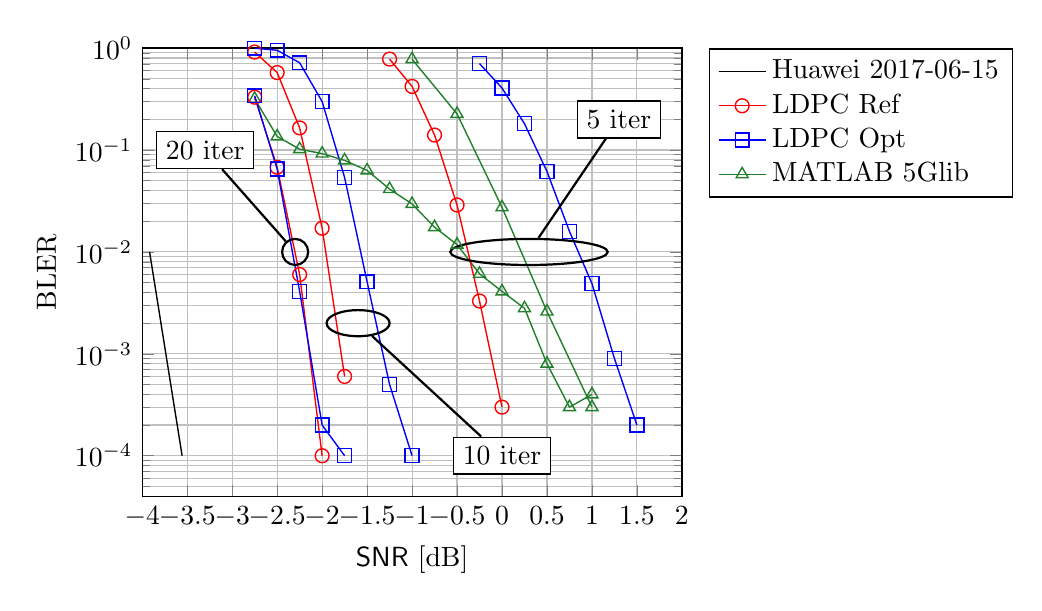
\begin{tikzpicture}
  \tikzstyle{every pin}=[fill=white,draw=black]
    \pgfplotsset{every axis legend/.append style={
        cells={anchor=west}, at={(1.05,1)}, anchor=north west}}
 %   \pgfplotsset{every axis plot/.append style={smooth}}
    \pgfplotsset{every axis/.append style={line width=0.5pt}}
    \pgfplotsset{every axis/.append style={mark options=solid, mark size=2.5pt}}

    \begin{semilogyaxis}[title={}, xlabel={$\SNR$ [dB]}, ylabel={BLER},
      grid={both}, xmin=-4, xmax=2, xtick={-4,-3.5,...,2}, ymin=0,
      ymax=1,ytickten={-5,-4,-3,-2,-1,0},legend columns=1]

      % HUAWEI merged BG2 2017-06-15
      \addplot[black, solid] plot coordinates { (-3.91839,0.01) (-3.5567,0.0001) };

      % Kien's 2-layer 16bit code
      \addplot[red, solid, mark=o] plot coordinates { (-2.750000,0.915500) (-2.500000,0.576000) (-2.250000,0.165000) (-2.000000,0.017100) (-1.750000,0.000600) (-1.500000,0.000000) (-1.250000,0.000000) (-1.000000,0.000000)};

      % LDPC opt with 16bit BN processing
      \addplot[blue, solid, mark=square] plot coordinates { (-2.750000,0.998600) (-2.500000,0.953600) (-2.250000,0.718800) (-2.000000,0.299300) (-1.750000,0.053700) (-1.500000,0.005100) (-1.250000,0.000500) (-1.000000,0.000100)};

      % Matlab
      \addplot[green, solid, mark=triangle] plot coordinates {(-2.750000,0.318200) (-2.500000,0.135900) (-2.250000,0.102000) (-2.000000,0.092300) (-1.750000,0.079200) (-1.500000,0.063100) (-1.250000,0.041400) (-1.000000,0.029600) (-0.750000,0.017500) (-0.500000,0.011800) (-0.250000,0.006100) (0.000000,0.004100) (0.250000,0.002800) (0.500000,0.000800) (0.750000,0.000300) (1.000000,0.000400) };


%      \addplot[blue, solid, mark=triangle] plot coordinates {(-2.750000,0.997600) (-2.500000,0.961600) (-2.250000,0.815200) (-2.000000,0.628800) (-1.750000,0.586200) (-1.500000,0.572800) (-1.250000,0.507600) (-1.000000,0.376700) (-0.750000,0.262000) (-0.500000,0.157100) (-0.250000,0.087100) (0.000000,0.045400) (0.250000,0.021000) (0.500000,0.010000) (0.750000,0.004400) (1.000000,0.002600) (1.250000,0.000700) (1.500000,0.000500) (1.750000,0.000000) (2.000000,0.000000) (2.250000,0.000000) (2.500000,0.000000) (2.750000,0.000000) (3.000000,0.000000)};

      % 20 iterations
      \addplot[red, solid, mark=o] plot coordinates { (-2.750000,0.330300) (-2.500000,0.067800) (-2.250000,0.006000) (-2.000000,0.000100) (-1.750000,0.000000) (-1.500000,0.000000) (-1.250000,0.000000) (-1.000000,0.000000)};

      \addplot[blue, solid, mark=square] plot coordinates {(-2.750000,0.341300) (-2.500000,0.065100) (-2.250000,0.004100) (-2.000000,0.000200) (-1.750000,0.000100) (-1.500000,0.000000) (-1.250000,0.000000) (-1.000000,0.000000)};

      % 5 iterations
\addplot[red, solid, mark=o] plot coordinates {(-1.250000,0.781300) (-1.000000,0.421000) (-0.750000,0.140400) (-0.500000,0.028900) (-0.250000,0.003300) (0.000000,0.000300) (0.250000,0.000000) (0.500000,0.000000)};
\addplot[blue, solid, mark=square] plot coordinates {(-0.250000,0.705000) (0.000000,0.406200) (0.250000,0.181300) (0.500000,0.061600) (0.750000,0.015900) (1.000000,0.004900) (1.250000,0.000900) (1.500000,0.000200)};
\addplot[green, solid, mark=triangle] plot coordinates {(-1.000000,0.778900) (-0.500000,0.226400) (0.000000,0.027400) (0.500000,0.002600) (1.000000,0.000300) };

% 30 iterations
% \addplot[blue, dashed, mark=square] plot coordinates {(-3.000000,0.623800) (-2.750000,0.224100) (-2.500000,0.031600) (-2.250000,0.001100) (-2.000000,0.000000)};


\draw (axis cs:-3.3,0.1)  node[fill=white,draw=black] (pint0) {20 iter};
\draw (axis cs:-2.3,0.01) node[draw,black,thick,ellipse,minimum height=0.3cm] (ell0) {}; \draw[black,thick] (pint0) -- (ell0);

\draw (axis cs:0,0.0001)   node[fill=white,draw=black] (pint1) {10 iter};
\draw (axis cs:-1.6,0.002) node[draw,black,thick,ellipse,minimum width=0.8cm] (ell1) {}; \draw[black,thick] (pint1) -- (ell1);

\draw (axis cs:1.3,0.2)  node[fill=white,draw=black] (pint2) {5 iter};
\draw (axis cs:0.3,0.01) node[draw,black,thick,ellipse,minimum width=2cm] (ell2) {}; \draw[black,thick] (pint2) -- (ell2);


      \legend{ {Huawei 2017-06-15}\\
               {LDPC Ref}\\
               {LDPC Opt}\\
               {MATLAB 5Glib}\\};

    \end{semilogyaxis}
  \end{tikzpicture}
  \caption{BLER vs. SNR, BG2, Rate=1/5, \{5,10,20\} Iterations, B=1280.}
  \label{fig:bler-bg2-15}
\end{figure}

From Figure \ref{fig:bler-bg2-15} it can be observed that the reference decoder outperforms the current implementation significantly for low to medium number of iterations. The reason is the implementation of 2 layers in the reference decoder, which results in faster convergence for punctured codes and hence requires less iterations to achieve a given BLER target. Note that there is a large performance loss of nearly 6 dB at BLER $10^{-2}$ between the Huawei reference and the current optimized decoder implementation with 5 iterations.

Moreover, there is a gap of about 1.5 dB between the results provided by Huawei and the current decoder with 20 iterations. The reason is the min-sum approximation algorithm used in both the reference decoder and the current implementation. The gap can be closed by using a tighter approximation like the min-sum with normalization or the lambda-min approach. Moreover, the gap closes for higher code rates which can be observed from Figure \ref{fig:bler-bg2-r23}. The gap is only about 0.6 dB for 50 iterations.

Concerning the LDPC decoder provided by MATLAB, the performance appears to be rather inconsistent. For 5 iterations, the MATLAB decoder outperforms the optimized decoder most likely due to a tighter approximation used in the check node processing. However, it is inferior to the reference algorithm which suggests that the MATLAB decoder is not optimized for punctured LDPC codes, i.e. no layered processing. For 50 iterations the MATLAB LDPC decoder shows a strange behavior, the slope of the BLER curve is not as expected. This suggests that there might be some internal decoder problems with the NR base graph 2.


\begin{figure}[ht]
  \centering
  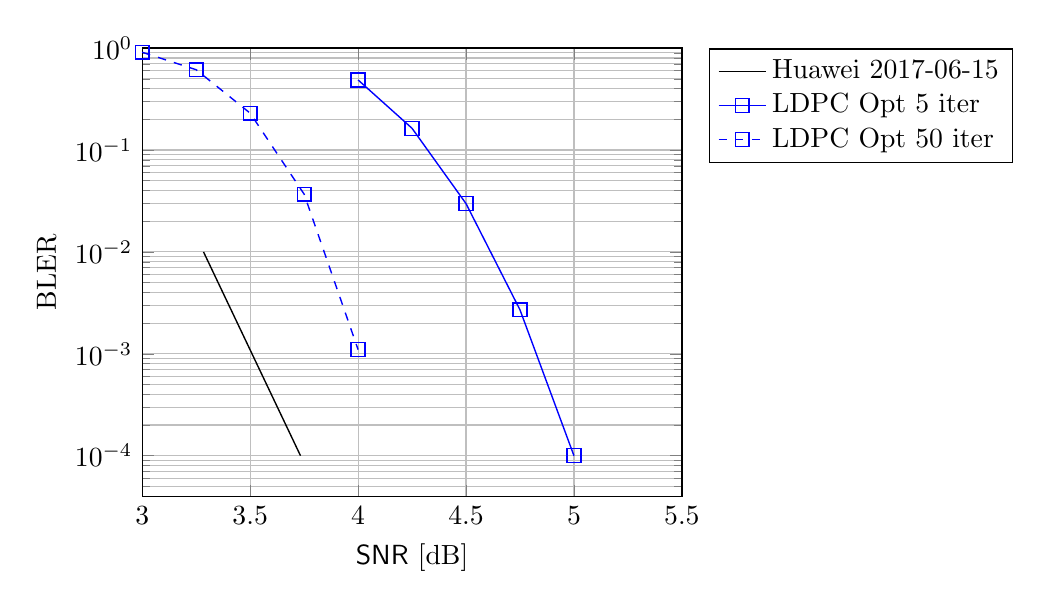
\begin{tikzpicture}
  \tikzstyle{every pin}=[fill=white,draw=black]
    \pgfplotsset{every axis legend/.append style={
        cells={anchor=west}, at={(1.05,1)}, anchor=north west}}
 %   \pgfplotsset{every axis plot/.append style={smooth}}
    \pgfplotsset{every axis/.append style={line width=0.5pt}}
    \pgfplotsset{every axis/.append style={mark options=solid, mark size=2.5pt}}

    \begin{semilogyaxis}[title={}, xlabel={$\SNR$ [dB]}, ylabel={BLER},
      grid={both}, xmin=3, xmax=5.5, xtick={3,3.5,...,5.5}, ymin=0,
      ymax=1,ytickten={-5,-4,-3,-2,-1,0},legend columns=1]

      % Kien's 2-layer 16bit code
      %\addplot[red, solid] plot coordinates { (-2.750000,0.915500) (-2.500000,0.576000) (-2.250000,0.165000) (-2.000000,0.017100) (-1.750000,0.000600) (-1.500000,0.000000) (-1.250000,0.000000) (-1.000000,0.000000)};

      % Huawei
      \addplot[black, solid] plot coordinates { (3.28392,0.01) (3.73319,0.0001) };

      % LDPC opt with 16bit BN processing
      \addplot[blue, solid, mark=square] plot coordinates {(4.000000,0.487500) (4.250000,0.163400) (4.500000,0.029800) (4.750000,0.002700) (5.000000,0.000100)};

      %\addplot[blue, dashed, mark=triangle] plot coordinates {(4.000000,0.487500) (4.250000,0.163700) (4.500000,0.030000) (4.750000,0.002900) (5.000000,0.000100)};

      \addplot[blue, dashed, mark=square] plot coordinates {(3.000000,0.911600) (3.250000,0.614100) (3.500000,0.230100) (3.750000,0.036900) (4.000000,0.001100) (4.250000,0.000000) (4.500000,0.000000)};


      \legend{ {Huawei 2017-06-15}\\
               {LDPC Opt 5 iter}\\
               {LDPC Opt 50 iter}\\};

    \end{semilogyaxis}
  \end{tikzpicture}
  \caption{BLER vs. SNR, BG2, Rate=2/3, \{5,50\} Iterations, B=1280.}
  \label{fig:bler-bg2-r23}
\end{figure}

Figure \ref{fig:bler-bg1-r89} shows the performance of BG1 with largest block size of $B=8448$ and highest code rate $R=8/9$.

\begin{figure}[ht]
  \centering
  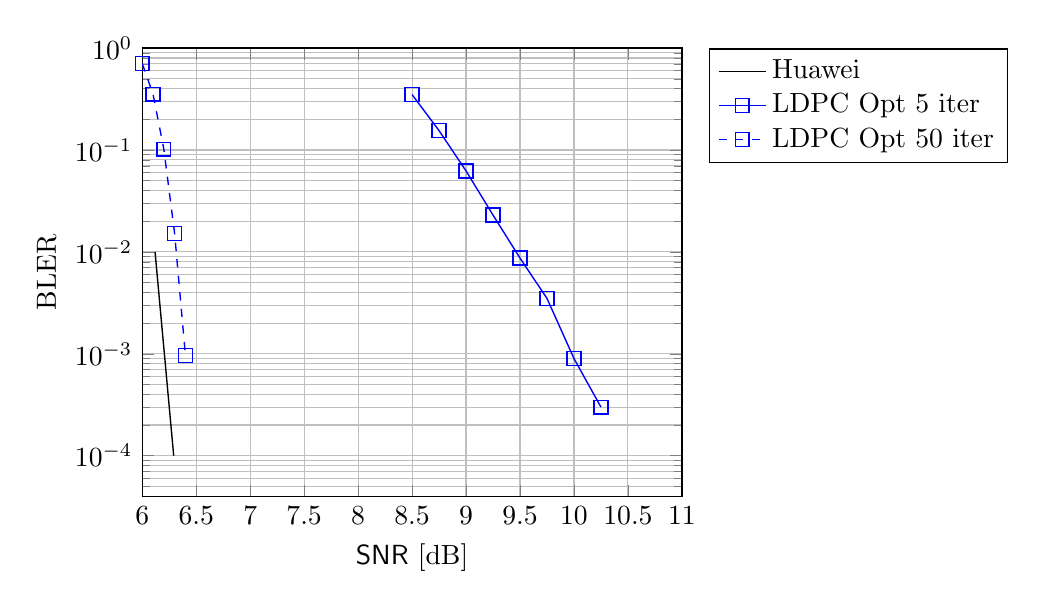
\begin{tikzpicture}
  \tikzstyle{every pin}=[fill=white,draw=black]
    \pgfplotsset{every axis legend/.append style={
        cells={anchor=west}, at={(1.05,1)}, anchor=north west}}
 %   \pgfplotsset{every axis plot/.append style={smooth}}
    \pgfplotsset{every axis/.append style={line width=0.5pt}}
    \pgfplotsset{every axis/.append style={mark options=solid, mark size=2.5pt}}

    \begin{semilogyaxis}[title={}, xlabel={$\SNR$ [dB]}, ylabel={BLER},
      grid={both}, xmin=6, xmax=11, xtick={6,6.5,...,11}, ymin=0,
      ymax=1,ytickten={-5,-4,-3,-2,-1,0},legend columns=1]

      % Huawei
      \addplot[black, solid] plot coordinates { (6.118717,0.01) (6.291449,0.0001) };

      % LDPC opt 5 iter
      \addplot[blue, solid, mark=square] plot coordinates {(8.500000,0.350000) (8.750000,0.155100) (9.000000,0.062400) (9.250000,0.023000) (9.500000,0.008700) (9.750000,0.003500) (10.000000,0.000900) (10.250000,0.000300) };

      % LDPC opt 50 iter
      \addplot[blue, dashed, mark=square] plot coordinates {(6.000000,0.705333) (6.100000,0.353367) (6.200000,0.102100) (6.300000,0.015133) (6.400000,0.000967) (6.500000,0.000000)};


      \legend{ {Huawei}\\
               {LDPC Opt 5 iter}\\
               {LDPC Opt 50 iter}\\};

    \end{semilogyaxis}
  \end{tikzpicture}
  \caption{BLER vs. SNR, BG1, Rate=8/9 \{5,50\} Iterations, B=8448.}
  \label{fig:bler-bg1-r89}
\end{figure}

From \ref{fig:bler-bg1-r89} it can be observed that the performance gap is only about 0.2 dB if 50 iterations are used. However, for 5 iterations there is still a significant performance loss of about 3.4 dB at BLER $10^{-2}$.

\newpage
\subsection{Decoding Latency}
\label{sec:decoding-time}

This section provides results in terms of decoding latency. That is, the time it takes the decoder to to finish decoding for a given number of iterations. To measure the run time of the decoder we use the OAI tool \texttt{time\_meas.h}. The clock frequency is about 2.9 GHZ, decoder is run on a single core and the results are averaged over $10\,000$ blocks.

The results in Table \ref{tab:lat-bg2-r15} show the impact of the number of iterations on the decoding latency. It can be observed that the latency roughly doubles if the number of iterations are doubled.

\begin{table}[ht]
  \centering
  \begin{tabular}{lrrr}
    \toprule
    \textbf{Function} & \textbf{Time [$\mu s$] (5 it)} & \textbf{Time [$\mu s$] (10 it)} & \textbf{Time [$\mu s$] (20 it)}\\
    \midrule
    \texttt{llr2llrProcBuf} & 1.1   & 1.1   & 1.1   \\
    \texttt{llr2CnProcBuf}  & 12.4  & 12.0  & 12.0  \\
    \texttt{cnProc}         & 11.7  & 22.1  & 43.5  \\
    \texttt{bnProcPc}       & 6.6   & 12.1  & 23.8  \\
    \texttt{bnProc}         & 4.2   & 8.1   & 16.2  \\
    \texttt{cn2bnProcBuf}   & 61.3  & 118.3 & 234.9 \\
    \texttt{bn2cnProcBuf}   & 38.1  & 82.5  & 172.3 \\
    \texttt{llrRes2llrOut}  & 3.5   & 3.4   & 3.4   \\
    \texttt{llr2bit}        & 0.2   & 0.1   & 0.1   \\
    \midrule
    \textbf{Total}          & \textbf{139.4} & \textbf{260.3} & \textbf{508.4} \\
    \bottomrule
  \end{tabular}
  \caption{BG2, Z=128, R=1/5, B=1280, LDPC Opt}
  \label{tab:lat-bg2-r15}
\end{table}

Table \ref{tab:lat-bg2-i5} shows the impact of the code rate on the latency for a given block size and 5 iterations. It can be observed that the performance gain from code rate 1/3 to 2/3 is about a factor 2.

\begin{table}[ht]
  \centering
  \begin{tabular}{lrrr}
    \toprule
    \textbf{Function} & \textbf{Time [$\mu s$] (R=1/5)} & \textbf{Time [$\mu s$] (R=1/3)} & \textbf{Time [$\mu s$] (R=2/3)}\\
    \midrule
    \texttt{llr2llrProcBuf} & 3.2   & 2.9   & 2.6   \\
    \texttt{llr2CnProcBuf}  & 36.5  & 25.4  & 14.8  \\
    \texttt{cnProc}         & 33.6  & 25.2  & 13.3  \\
    \texttt{bnProcPc}       & 17.6  & 10.2  & 4.5   \\
    \texttt{bnProc}         & 8.5   & 5.4   & 2.5   \\
    \texttt{cn2bnProcBuf}   & 175.3 & 110.6 & 50.7  \\
    \texttt{bn2cnProcBuf}   & 106.6 & 71.2  & 36.1  \\
    \texttt{llrRes2llrOut}  & 10.2  & 6.3   & 3.3   \\
    \texttt{llr2bit}        & 0.4   & 0.2   & 0.1   \\
    \midrule
    \textbf{Total}          & \textbf{392.4} & \textbf{258.0} & \textbf{128.2} \\
    \bottomrule
  \end{tabular}
  \caption{BG2, Z=384, B=3840, LDPC Opt, 5 iterations}
  \label{tab:lat-bg2-i5}
\end{table}

Table \ref{tab:lat-bg1-i5} shows the results for BG1, larges block size and different code rates. The latency difference betwee code rate 1/3 and code rate 2/3 is less than half because upper left corner of the PCM is more dense than the rest of the PCM.

\begin{table}[ht]
  \centering
  \begin{tabular}{lrrr}
    \toprule
    \textbf{Function} &  \textbf{Time [$\mu s$] (R=1/3)} & \textbf{Time [$\mu s$] (R=2/3)} & \textbf{Time [$\mu s$] (R=8/9)}\\
    \midrule
    \texttt{llr2llrProcBuf}  & 5.5   & 4.9   & 4.6  \\
    \texttt{llr2CnProcBuf}   & 60.6  & 34.1  & 24.4 \\
    \texttt{cnProc}          & 102.0 & 74.1  & 56.0 \\
    \texttt{bnProcPc}        & 26.0  & 11.0  & 6.4  \\
    \texttt{bnProc}          & 15.7  & 7.4   & 4.5  \\
    \texttt{cn2bnProcBuf}    & 291.0 & 140.8 & 83.1 \\
    \texttt{bn2cnProcBuf}    & 193.6 & 100.5 & 63.0 \\
    \texttt{llrRes2llrOut}   & 13.3  & 6.9   & 5.2  \\
    \texttt{llr2bit}         & 0.4   & 0.2   & 0.2  \\
    \midrule
    \textbf{Total}           & \textbf{708.9} & \textbf{380.6} & \textbf{248.1}\\
    \bottomrule
  \end{tabular}
  \caption{BG1, Z=384, B=8448, LDPC Opt, 5 iterations}
  \label{tab:lat-bg1-i5}
\end{table}

From the above results it can be observed that the data transfer between CNs and BNs takes up a significant amount of the run time. However, the performance gain due to AVX instructions in both CN and BN processing is significantly larger than the penalty incurred by the data transfers.

\section{Parity Check and early stopping Criteria}
It is often unnecessary to carry out the maximum number of iterations. After each iteration a parity check \eqref{eq:29} can be computed and if a valid code word is found the decoder can stop. This functionality has been implemented and the additional overhead is reasonable. The PC is carried out in the CN processing buffer and the calculation complexity itself is negligible. However, for the processing it is necessary to move the BN results to the CN buffer which takes time, the overall overhead is at most $10\%$ compared to an algorithm without early stopping criteria with the same number of iterations. The PC has to be activated via the define \texttt{NR\_LDPC\_ENABLE\_PARITY\_CHECK}.


\section{Conclusion}
\label{sec:conclusion}

The results in the previous sections show that the current optimized LDPC implementation full-fills the requirements in terms of decoding latency for low to medium number of iterations at the expanse of a significant loss in BLER performance. To improve BLER performance, it is recommended to implement a layered algorithm and a min-sum algorithm with normalization. Further improvements upon the current implementation are detailed in the next section.

\newpage
\section{Future Work}
\label{sec:future-work}

The improvements upon the current LDPC decoder implementation can be divided into two categories:
\begin{enumerate}
\item Improved BLER performance
\item Reduced decoding latency
\end{enumerate}

\subsection{Improved BLER Performance}
\label{sec:impr-bler-perf}

The BLER performance can be improved by using a tighter approximation than the min-sum approximation. For instance, the min-sum algorithm can be improved by adding a correction factor in the CN processing . The min-sum approximation in \eqref{eq:40} is modified as
\begin{equation}
  \label{eq:50}
  r_{ji} = \prod_{j'\in\Bcal_i\setminus j}\sgn q_{ij'}\min_{j'\in\Bcal_i\setminus j} |q_{ij'}| + w(q_{ij'})
\end{equation}
The correction term $w(q_{ij'})$ is defined as
\begin{equation}
  \label{eq:51}
  w(q_{ij'}) =
  \begin{cases}
     c & \textrm{if}~  \\
    -c & \textrm{if}~ \\
     0 & \textrm{otherwise}
  \end{cases}
\end{equation}
where the constant $c$ is of order $0.5$ typically.

\subsection{Reduced Decoding Latency}
\label{sec:reduc-decod-latency}

The following improvements will reduce the decoding latency:

\begin{itemize}
\item Adapt to AVX512
\item Implement 2/3-layers for faster convergence
\end{itemize}

\paragraph{AVX512:}
The computations in the CN and BN processing can be further accelerated by using AVX512 instructions. This improvement will speed-up the CN and BN processing by a approximately a factor of 2.

\paragraph{Layered processing:}
The LDPC code in NR always punctures the first 2 columns of the base graph. Hence, the decoder inserts LLRs with value 0 at their place and needs to retrieve those bits during the decoding process. Instead of computing all the parity equations and then passing the results to the BN processing, it is beneficial to first compute parity equations where at most one punctured BN is connected to that CN. If two punctured BNs are connected than according to \eqref{eq:40}, the result will be again 0. Thus in a first sub-iteration those parity equation are computed and the results are send to BN processing which calculates the results using only those rows in the PCM. In the second sub-iteration the remaining check equation are used.
The convergence of this layered approach is much fast since the bit can be retrieved more quickly while the decoding complexity remains the same. Therefore, for a fixed number of iterations the layered algorithm will have a significantly better performance.

\newpage
\bibliographystyle{IEEEtran}
\bibliography{./references}

\end{document}

%%% Local Variables:
%%% mode: latex
%%% TeX-master: t
%%% End:
